  \pagebreak
  \subsection{Análisis de una señal modulada en amplitud}
    Las señales que son moduladas en amplitud (AM) poseen un espectro característico. Para poder visualizar
    el espectro de una señal AM se utiliza el circuito de la Figura~\ref{fig:ModuladorAM}. El mismo posee un
    circuito sintonizado o resonante, cuya frecuencia es $\mathbf{f_o = 50~kHz}$.

    \begin{figure}[H]
      \centering
      \frame{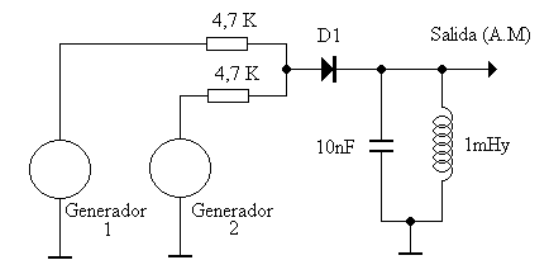
\includegraphics[width=0.48\textwidth]{Imagenes/ActividadPractica/4AnalisisDeUnaSeñalDeAM/CircuitoModAM.png}}
      \caption{Circuito de modulación en amplitud.}
      \label{fig:ModuladorAM}
    \end{figure}

    Con el generador \textbf{G1} se inyecta una señal senoidal que actúa como \textbf{portadora} de frecuencia 
    $\mathbf{f_c=50~kHz}$, y con el generador \textbf{G2} se inyecta la señal \textbf{modulante} de frecuencia
    $\mathbf{f_m=1~kHz}$, que puede ser senoidal, triangular o cuadrada. Las amplitudes utilizadas mantienen 
    una relación tal que la de la portadora sea el doble que la de modulante.

    \subsubsection{Señal senoidal como modulante}
      Se setea el generador G2 para que entregue una señal senoidal, que actúa como banda base. Dicha señal
      y la portadora se pueden ver en la Figura~\ref{fig:SeñalesParaAM1}.
      
      \begin{figure}[H]
        \centering
        \begin{subfigure}[H]{0.48\textwidth}
          \frame{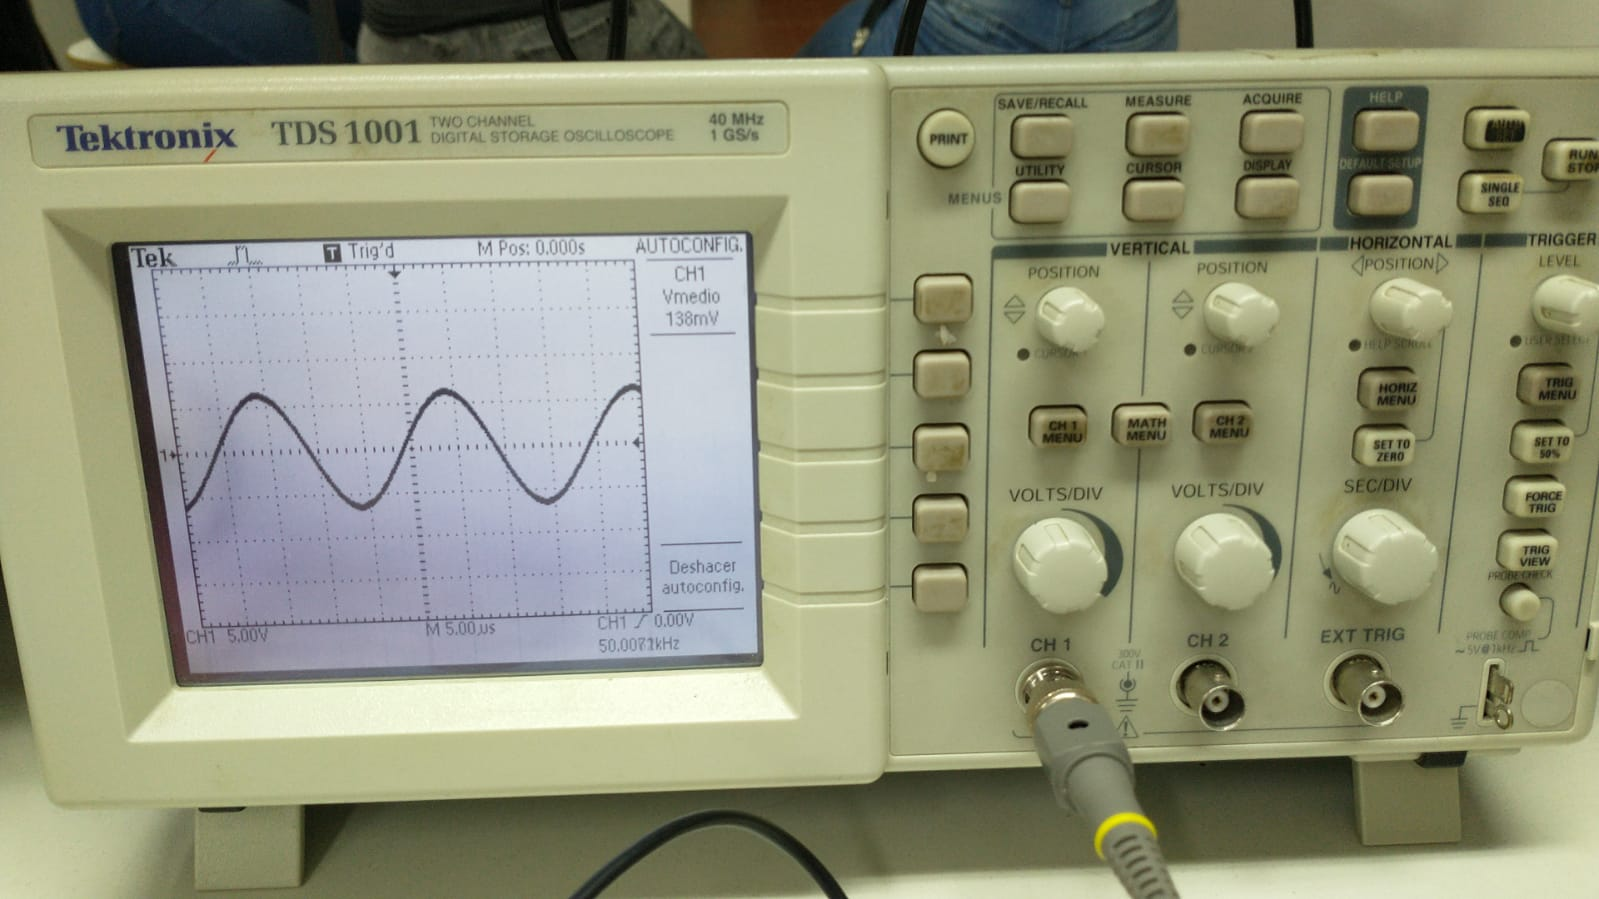
\includegraphics[width=\textwidth]{Imagenes/ActividadPractica/4AnalisisDeUnaSeñalDeAM/Exp4_G1Portadora_enTiempo.jpeg}}
          \caption{Portadora.}
          \label{fig:PortadoraEnTiempo}
        \end{subfigure}
        \hfill 
        \begin{subfigure}[H]{0.48\textwidth}
          \frame{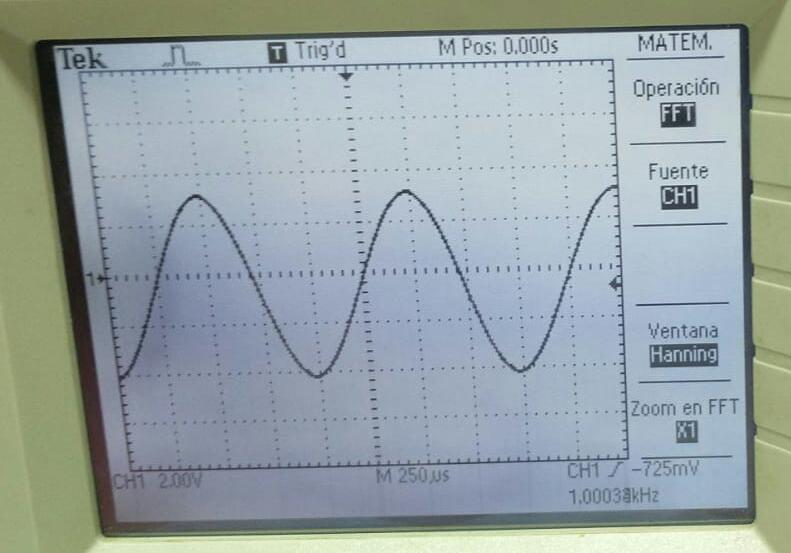
\includegraphics[width=\textwidth]{Imagenes/ActividadPractica/4AnalisisDeUnaSeñalDeAM/Exp4_G2SenoModulante_enTiempo.jpeg}}
          \caption{Banda base senoidal.}
          \label{fig:SenoModulanteEnTiempo}
        \end{subfigure}
      
        \caption{Señales utilizadas para modular en amplitud,}
        \label{fig:SeñalesParaAM1}
      \end{figure}
        
      
      Se elige una base de tiempos de $\mathbf{1~ms/div}$ y luego, el menú del trigger se setea de la siguiente manera:
      \textbf{Pendiente: +}, \textbf{Fuente: CH1}, \textbf{Modo: Auto}, \textbf{Acoplamiento: Rechazo AF}. Con
      todo esto, la imagen obtenida se encuentra en la Figura~\ref{fig:SeñalAM1EnTiempo}.
      
      \begin{figure}[H]
        \centering
        \frame{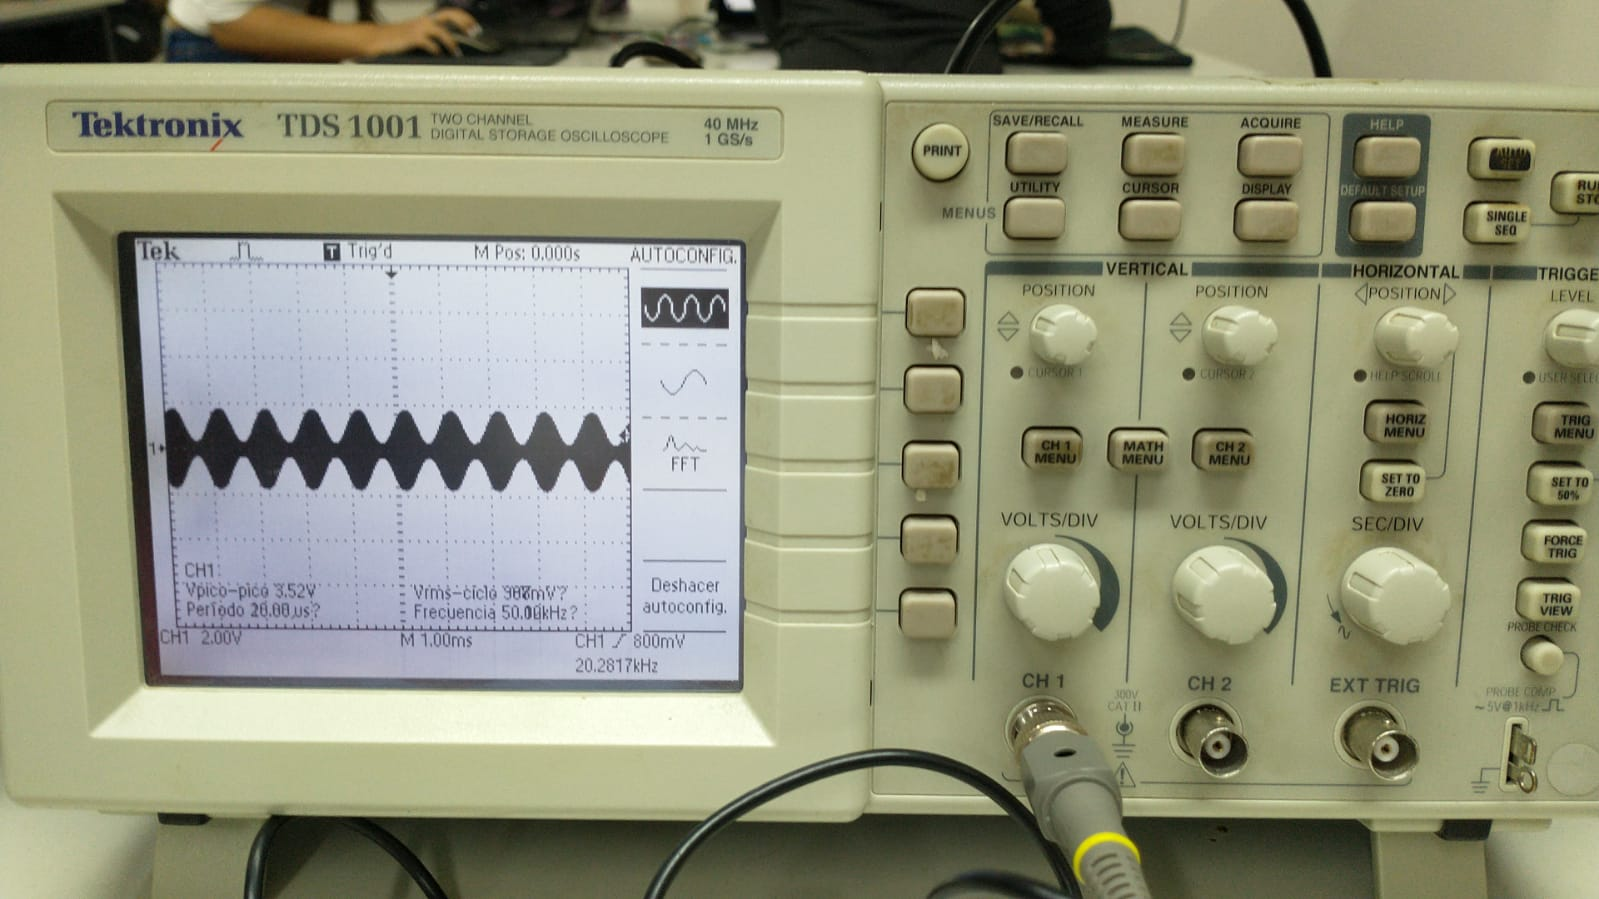
\includegraphics[width=0.48\textwidth]{Imagenes/ActividadPractica/4AnalisisDeUnaSeñalDeAM/Exp4_SeñalAM.jpeg}}
        \caption{Señal AM con seno como modulante.}
        \label{fig:SeñalAM1EnTiempo}
      \end{figure}

      Luego, en el menú matemático se eligen las siguientes opciones: \textbf{Operación: FFT}, \textbf{Fuente: CH1}, \textbf{Ventana: Hanning} y
      \textbf{Zoom x10}. Además. el modo de adquisición se pone en \textbf{Promedio} con 64 cuentas. A continuación, mediante el uso de 
      cursores, se procede a medir la frecuencias. Dichas mediciones se pueden apreciar en la Figura~\ref{fig:FreqAMSeno}, y los valores 
      se encuentran tabulados en la Tabla~\ref{tab:MedicionesFreqAMSeno}.

      \begin{figure}[H]
        \centering
        \begin{subfigure}[H]{0.48\textwidth}
          \frame{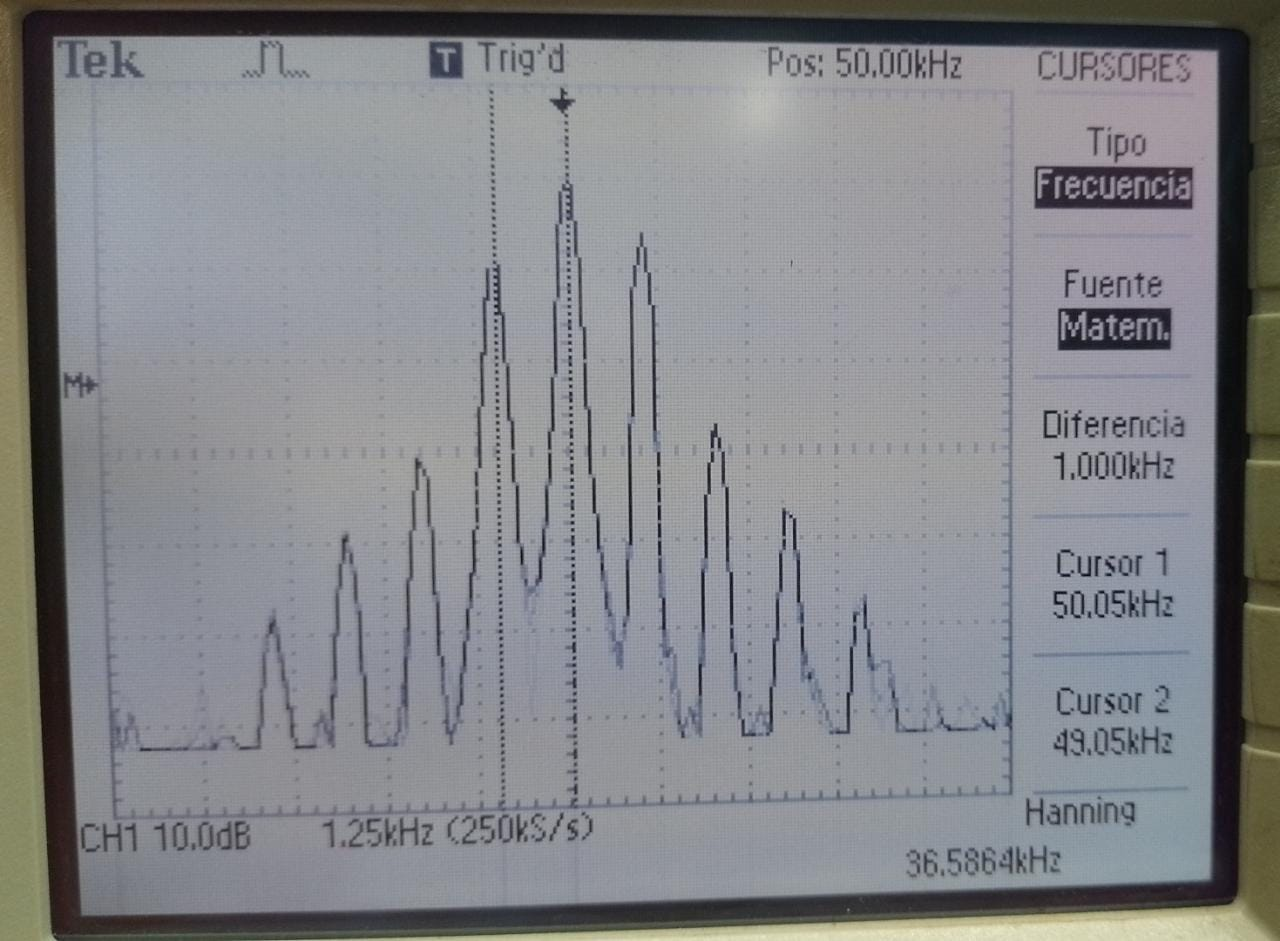
\includegraphics[width=\textwidth]{Imagenes/ActividadPractica/4AnalisisDeUnaSeñalDeAM/Exp4_SeñalAM_MedicionFreqBLInf.jpeg}}
          \caption{Frecuencia BLInf.}
          \label{fig:FreqBLInfAMSeno}
        \end{subfigure}
        \hfill 
        \begin{subfigure}[H]{0.48\textwidth}
          \frame{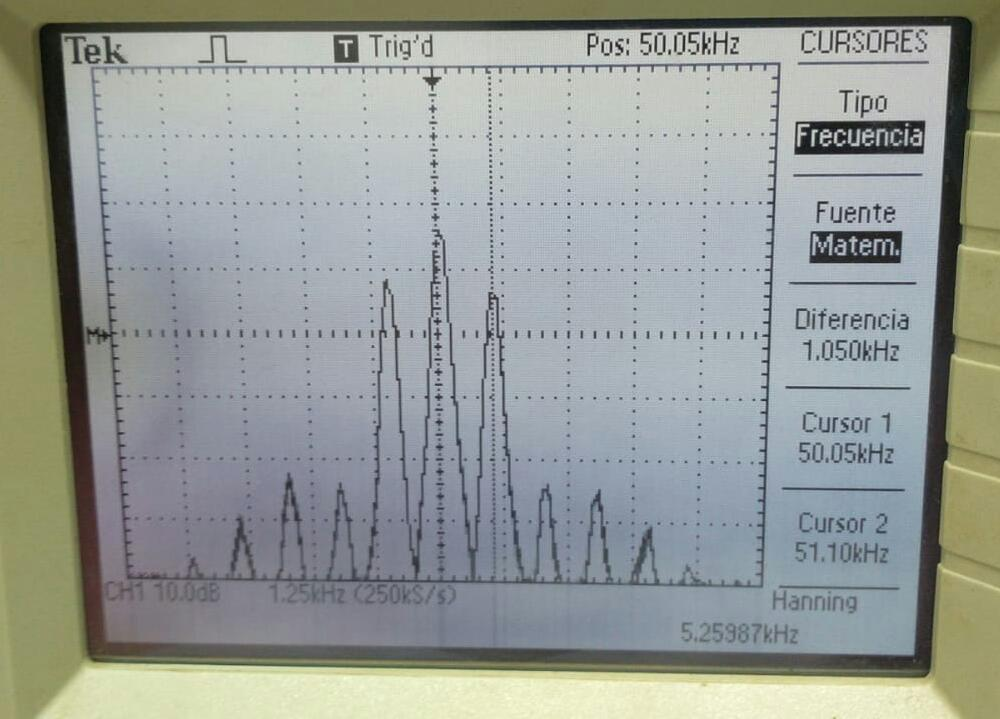
\includegraphics[width=\textwidth]{Imagenes/ActividadPractica/4AnalisisDeUnaSeñalDeAM/Exp4_SeñalAM_MedicionFreqBLSup.jpeg}}
          \caption{Frecuencia BLSup.}
          \label{fig:FreqBLSupAMSeno}
        \end{subfigure}
      
        \caption{Frecuencias de la señal AM con el seno como modulante.}
        \label{fig:FreqAMSeno}
      \end{figure}

      \begin{table}[H]
        \centering
      \begin{tabular}{cccc} \hline \hline
          $\mathbf{f_c} $        &   $\mathbf{f_{BLSup}}$   &   $\mathbf{f_{BLInf}}$    &   $\mathbf{f_m}$  \\ \hline
          $50,05~kHz$   &   $51,10~kHz$   &    $49,10~kHz$   &   $1,05~kHz$   \\ \hline \hline
        \end{tabular}
        \caption{Frecuencias medidas del espectro de la señal AM.}
        \label{tab:MedicionesFreqAMSeno}
      \end{table}

      De la misma forma, se procede a realizar mediciones de amplitud de la señal AM en cuestión. 

      \begin{figure}[H]
        \centering
        \begin{subfigure}[H]{0.48\textwidth}
          \frame{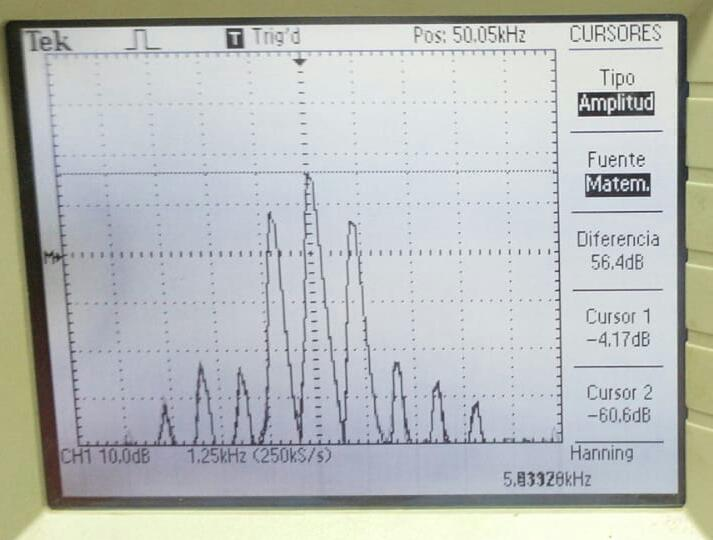
\includegraphics[width=\textwidth]{Imagenes/ActividadPractica/4AnalisisDeUnaSeñalDeAM/Exp4_SeñalAM_MedicionAmplPortadora.jpeg}}
          \caption{Amplitud BLInf.}
          \label{fig:AmplitudBLInfAMSeno}
        \end{subfigure}
        \hfill 
        \begin{subfigure}[H]{0.48\textwidth}
          \frame{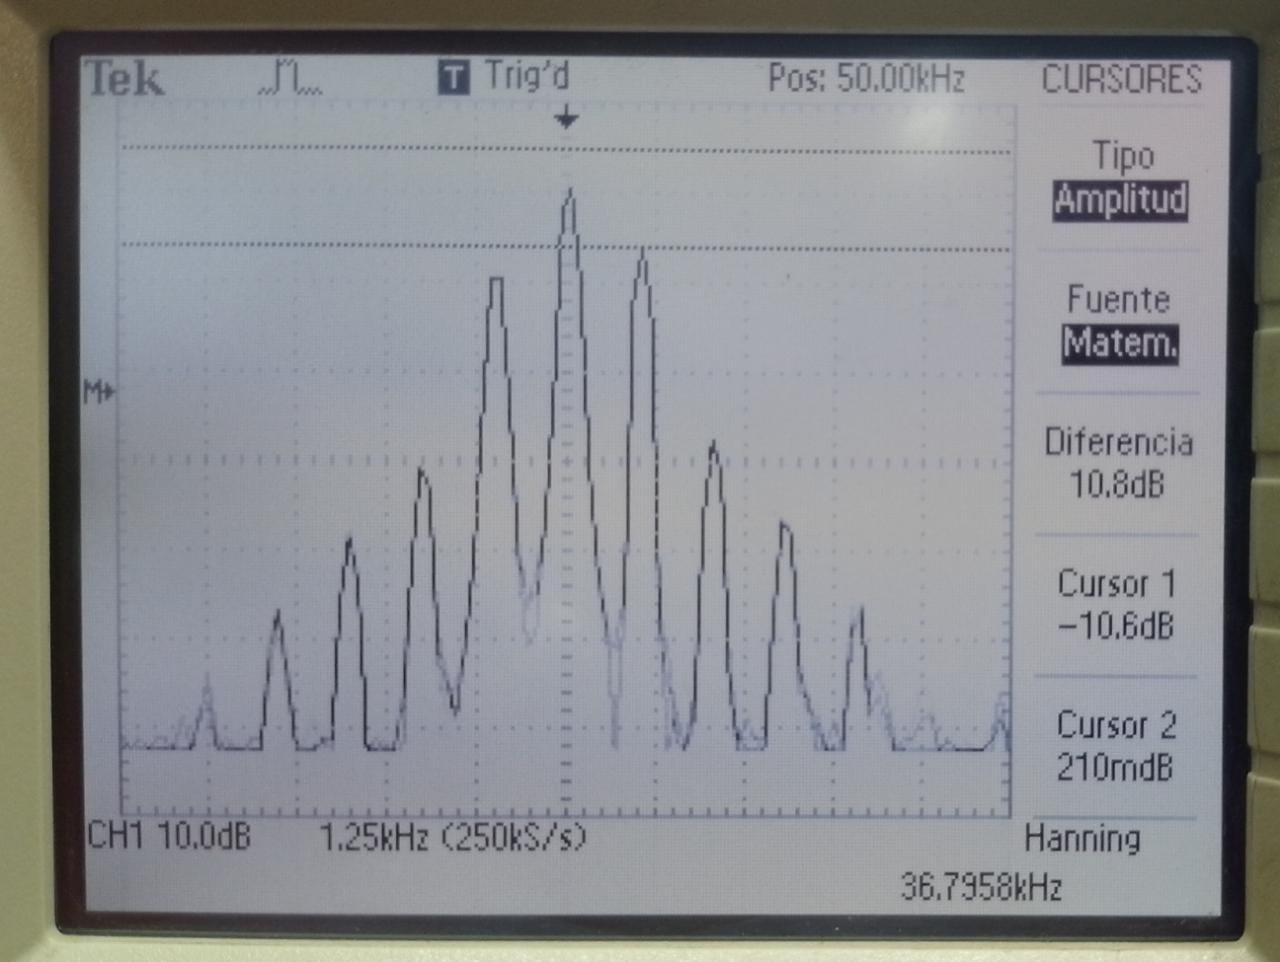
\includegraphics[width=\textwidth]{Imagenes/ActividadPractica/4AnalisisDeUnaSeñalDeAM/Exp4_SeñalAM_MedicionAmplBLSup.jpeg}}
          \caption{Amplitud BLSup.}
          \label{fig:AmpltiudBLSupAMSeno}
        \end{subfigure}
      
        \caption{Frecuencias de la señal AM con el seno como modulante.}
        \label{fig:AmplitudesAMSeno}
      \end{figure}

